\documentclass{article}

\usepackage{graphicx}
\usepackage{multicol}
\usepackage[center]{titlesec}
\usepackage{geometry}
%\usepackage{mathtools}



%
%\setlength{\columnseprule}{0.4pt}
%\setlength{\footskip}{20pt}
\usepackage{fancyhdr}
\fancyhf{}
\fancyhead[C]{Joe Brew $\bullet$ FDOH-Alachua $\bullet$ Ben Brew}
\fancyfoot[C]{  $\bullet$ Mosquito Surveillance Report \bullet$  }
\renewcommand\headrulewidth{1pt}
\renewcommand\footrulewidth{1pt}
\pagestyle{fancy}

%

\setlength{\columnsep}{1.5cm}
%\setlength{\columnseprule}{0.4pt}

%\MakeOuterQuote{"}



\graphicspath{ {C:/Users/BrewJR/Documents/fdoh/public/mosquito/reports/2014-11-07} }

%the next two lines adjust the third, centered section of the exec sum
\def\changemargin#1#2{\list{}{\rightmargin#2\leftmargin#1}\item[]}
\let\endchangemargin=\endlist 

\usepackage{Sweave}
\begin{document}
\Sconcordance{concordance:mosquitoReport.tex:mosquitoReport.Rnw:%
1 36 1 1 0 17 1 1 20 82 1 1 88 1 3 12 1 1 27 1 2 19 1 1 24 1 2 12 1 1 %
30 1 2 14 1 1 98 1 2 10 1 1 13 1 2 10 1 1 22 1 4 1 1 1 22 1 3 39 1}


\title{\textbf{Mosquito Surveillance Report}}
\author{Joe Brew and Ben Brew}


\maketitle
\tableofcontents

\vspace{40mm}

\begin{center}

\includegraphics[width=2cm]{doh}
\end{center}





\newgeometry{margin=5cm}
\fancyhfoffset[E,O]{0pt}


\vspace*{30mm}
%------------------------------------------
\section*{Executive Summary}
\addcontentsline{toc}{section}{Executive Summary}
%------------------------------------------
\hrulefill




\begin{multicols}{2} 
\setkeys{Gin}{width=0.49\textwidth}


%------------------------------------------
\subsection*{Most Recent Collection}
%------------------------------------------

As predicted, mosquito numbers remained low over recent weeks, ranging from 131 to 164 per trap through the most recent collection (October 21, 2014).  

\vfill
\columnbreak



%------------------------------------------
\subsection*{Forecast}
%------------------------------------------

We forecast that mosquito levels will remain low through next week (90\% confidence interval of 0-251 through November 14th). 



\end{multicols}
\setkeys{Gin}{width=1\textwidth}

\vspace{2mm}
%------------------------------------------
\subsection*{Predictive Model Validation}
%------------------------------------------


\begin{changemargin}{1.5cm}{1.5cm} 

At 158 specimens per trap, the most recent collection was similar to our prediction of 173, and well within the 90\% confidence interval for the range of prediction.

\end{changemargin}

\hrulefill


\newgeometry{margin=2.5cm}
\fancyhfoffset[E,O]{0pt}
%------------------------------------------
%\section*{Visual Overview}
%\addcontentsline{toc}{section}{Visual Overview}
%------------------------------------------


%------------------------------------------
\section*{Visual Overview}
\addcontentsline{toc}{section}{Visual Overview}
%------------------------------------------
\hrulefill

\begin{multicols}{2} 
\setkeys{Gin}{width=0.49\textwidth}



%------------------------------------------
\subsection*{Time}
\addcontentsline{toc}{subsection}{Time}
%------------------------------------------
The current mosquito population is lower than usual for this time of year (and significantly lower than last year's mid-September spike).
\begin{center}
%\begin{figure}
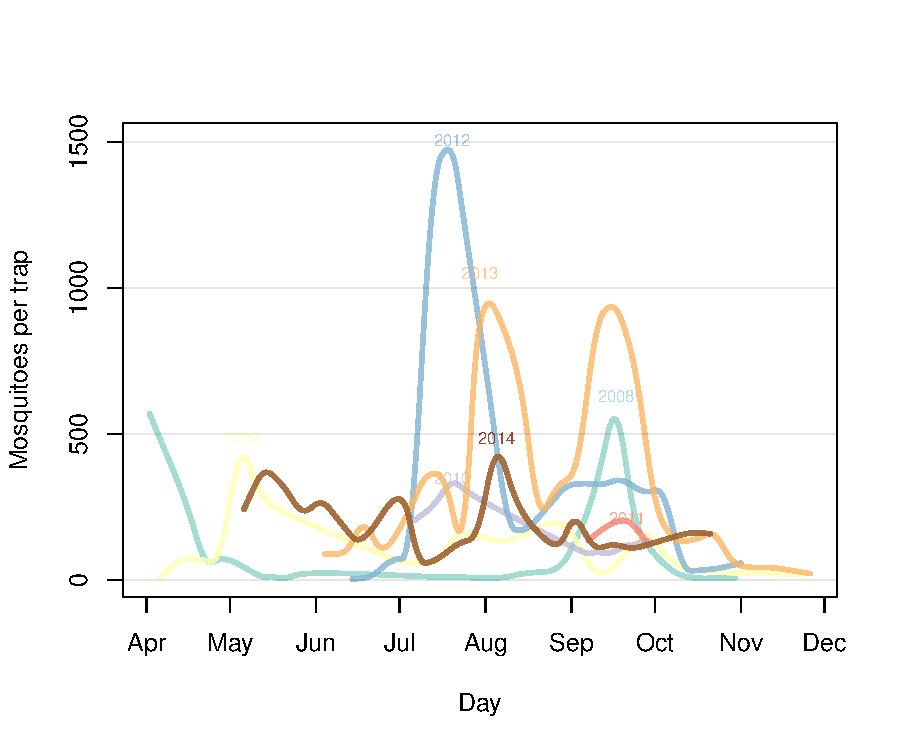
\includegraphics{mosquitoReport-002}
%\caption{Yearly comparison}
%\end{figure}
\end{center}


\vfill
\columnbreak
%------------------------------------------
\subsection*{Space}
\addcontentsline{toc}{subsection}{Space}
%------------------------------------------
Mosquitoes were largely scattered throughout the county, with a slight concentration in the northern traps.

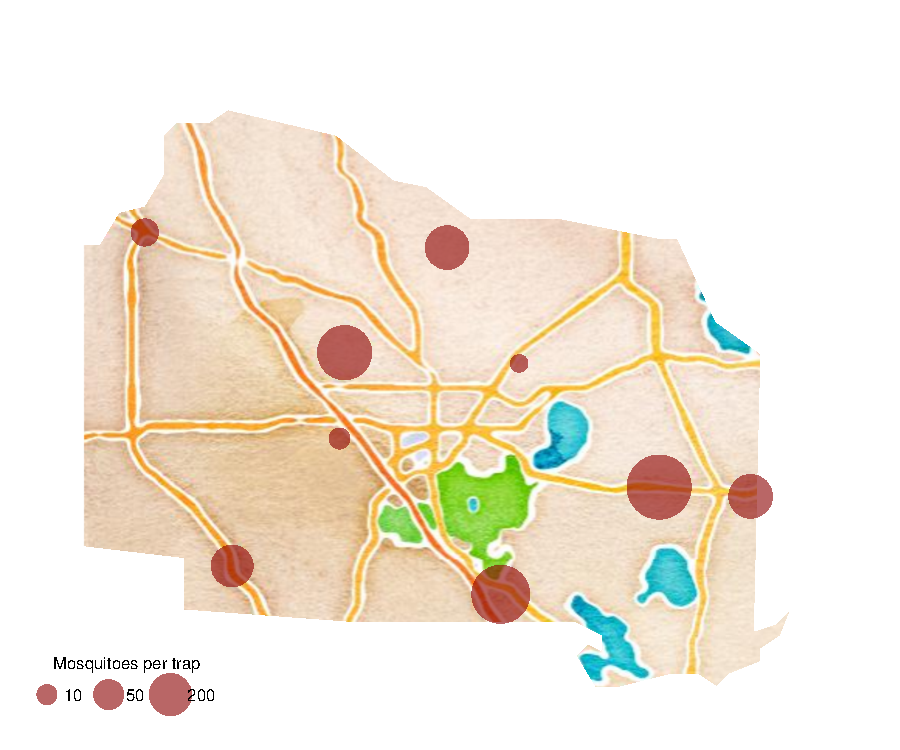
\includegraphics{mosquitoReport-003}

\end{multicols}
\setkeys{Gin}{width=1\textwidth}


%\hrulefill
\vspace{10mm}

\begin{multicols}{2} 
\setkeys{Gin}{width=0.49\textwidth}


\vfill
\columnbreak
%------------------------------------------
\subsection*{Normality}
\addcontentsline{toc}{subsection}{Normality}
%------------------------------------------
The most recent collection was at levels equivalent to approximately the 58th percentile of historical (2008-13) levels.

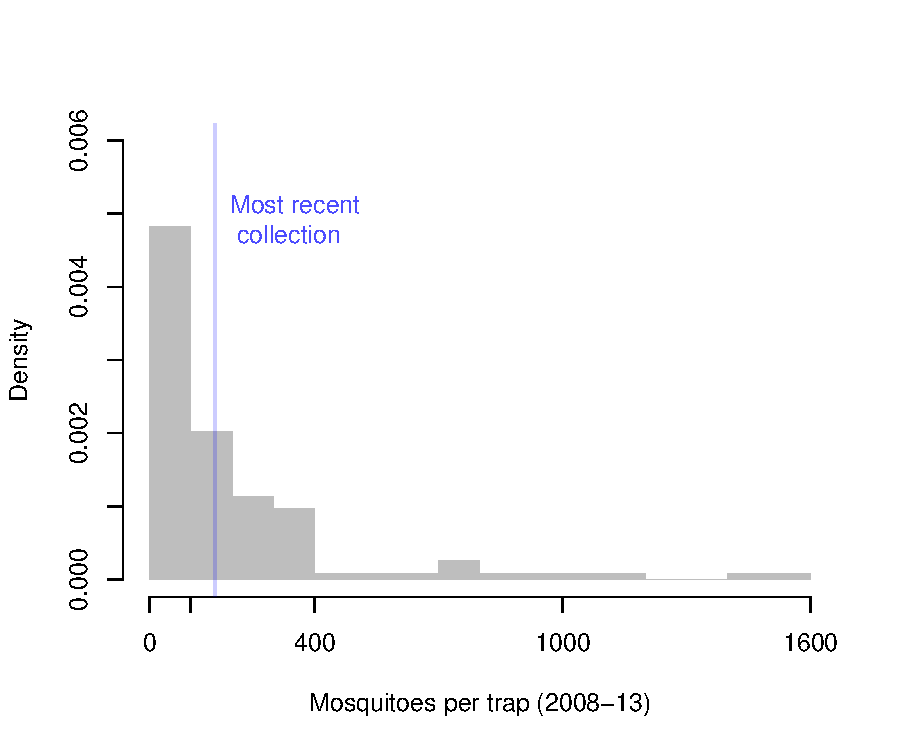
\includegraphics{mosquitoReport-004}

\vfill
\columnbreak



%------------------------------------------
\subsection*{Disease Vectors}
\addcontentsline{toc}{subsection}{Disease Vectors}
%------------------------------------------

Mosquitoes capable of carrying WNV are much more predominant now than at the beginning of the summer.

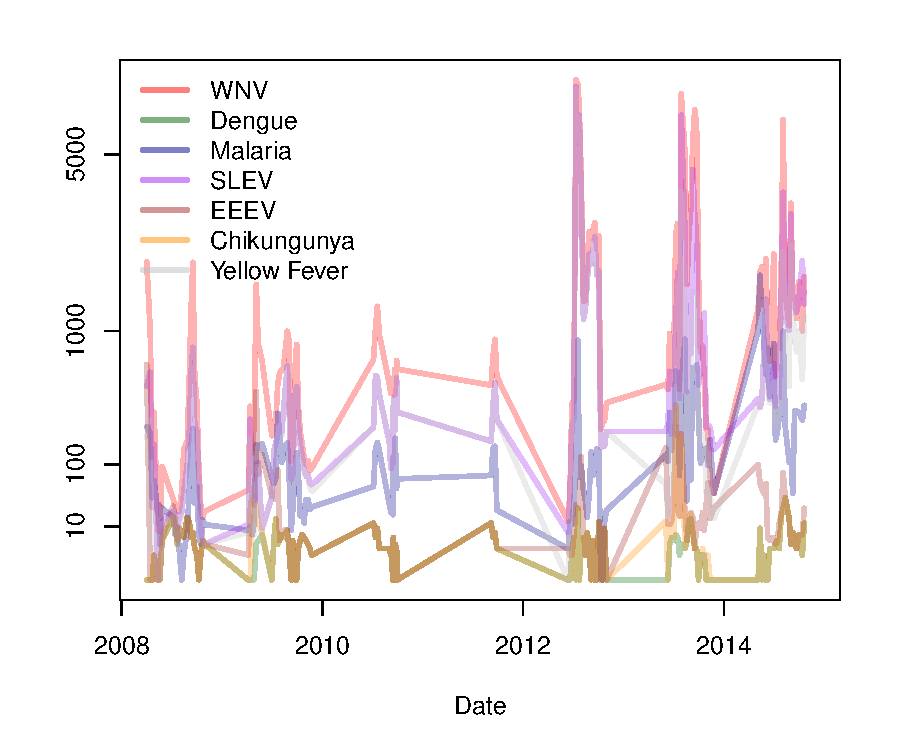
\includegraphics{mosquitoReport-005}

\vfill
\newpage
\end{multicols}
\setkeys{Gin}{width=1\textwidth}

%------------------------------------------
\section*{Forecast}
\addcontentsline{toc}{section}{Forecast}
%------------------------------------------
\hrulefill
\vspace{5mm}

\noindent We use recursive, quadratic linear regression modelling to forecast the average number of mosquitoes per trap up to 15 days in advance.\footnote{We are actively experimenting with non-parametric approaches to improve modelling accuracy, and expect to have a modified KNN model with better results by late September.}  

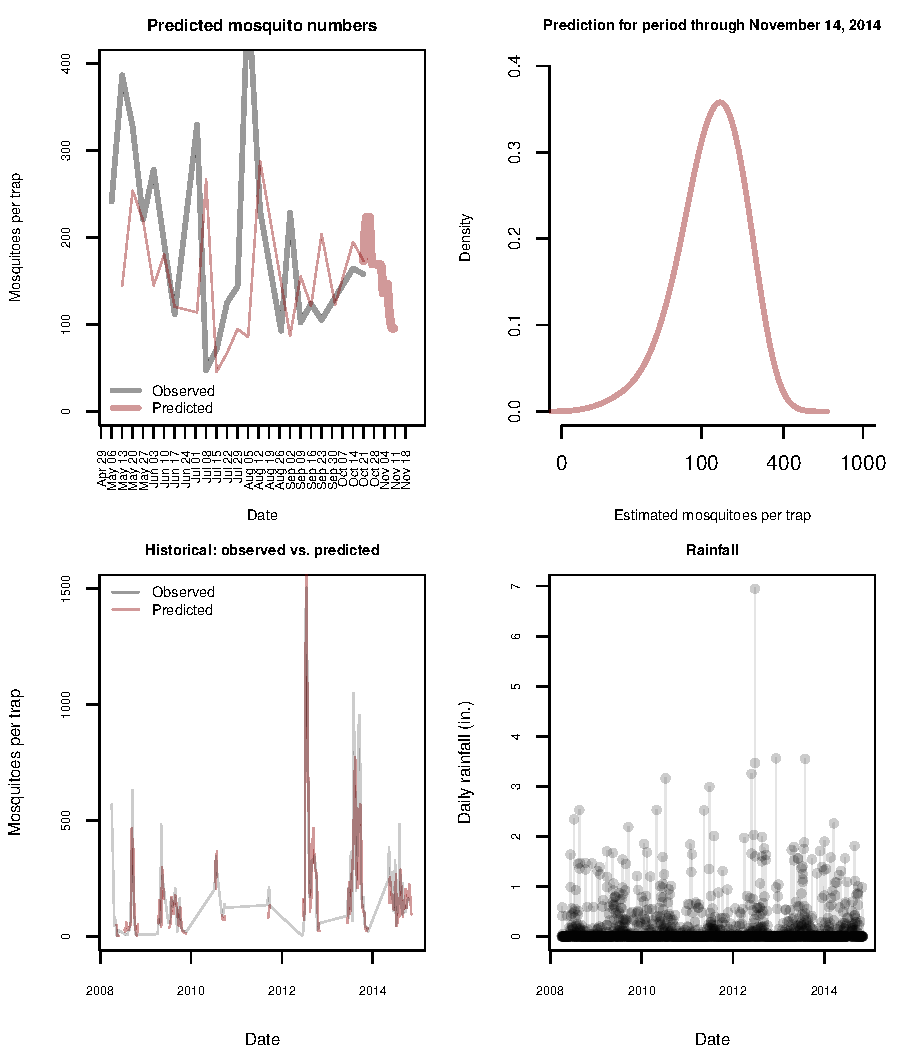
\includegraphics{mosquitoReport-006}


\newpage

%------------------------------------------
\section*{Vectors of Disease by Location}
\addcontentsline{toc}{section}{Vectors of Disease by Location}
%------------------------------------------
\hrulefill
\vspace{5mm}

Mosquito species cabale of carrying WNV and SLEV were most prevalent in recent trap collections.

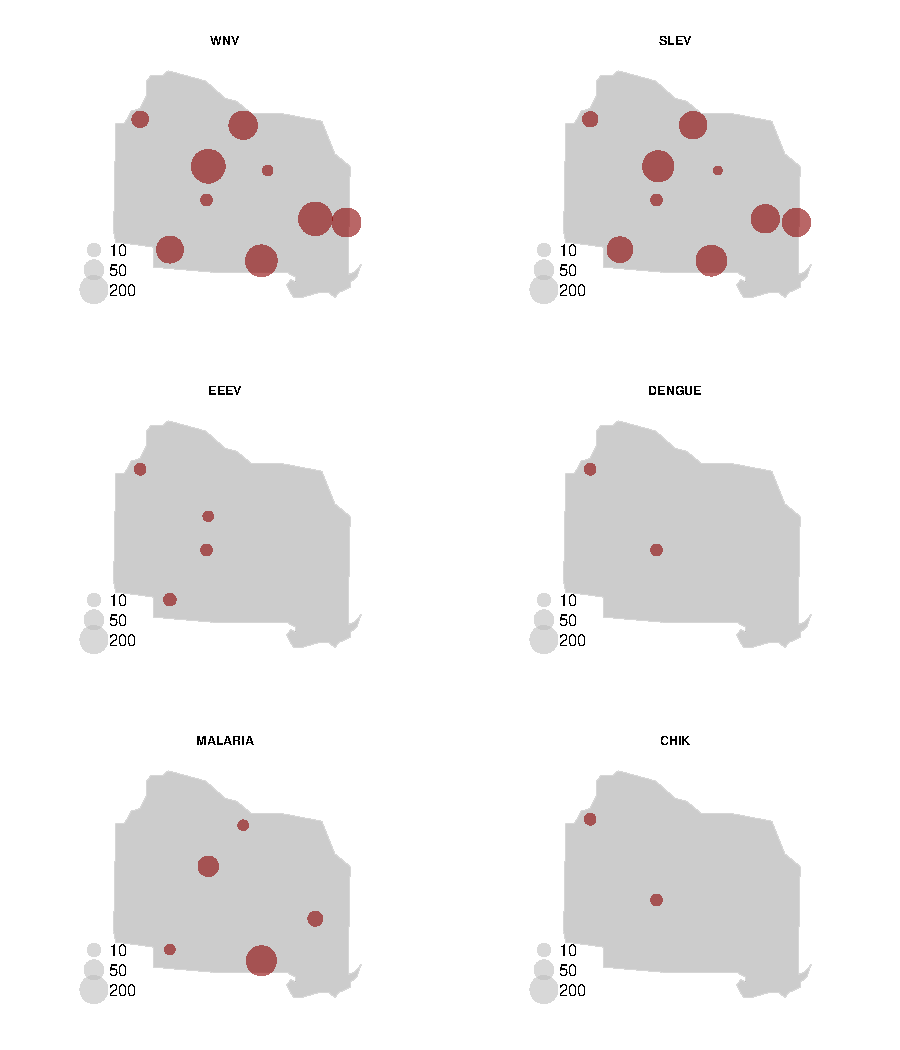
\includegraphics{mosquitoReport-007}


%------------------------------------------
\section*{Spatial interpolation maps}
\addcontentsline{toc}{section}{Spatial interpolation maps}
%------------------------------------------
\hrulefill
\vspace{5mm}

Mosquito species cabale of carrying WNV and SLEV were most prevalent in recent trap collections.

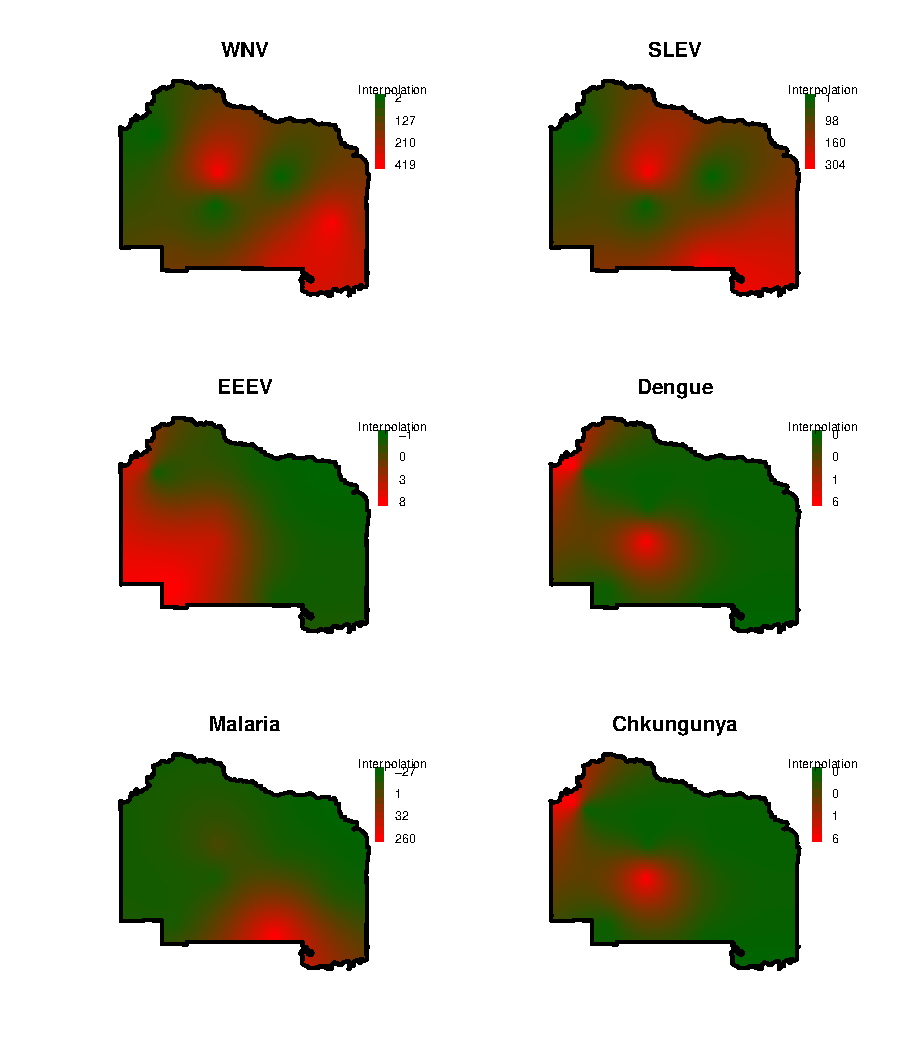
\includegraphics{mosquitoReport-008}


%------------------------------------------
\section*{Mosquito Types}
\addcontentsline{toc}{section}{Mosquito Types}
%------------------------------------------
\hrulefill
\vspace{5mm}

No species saw abnormal increases in recent weeks.  

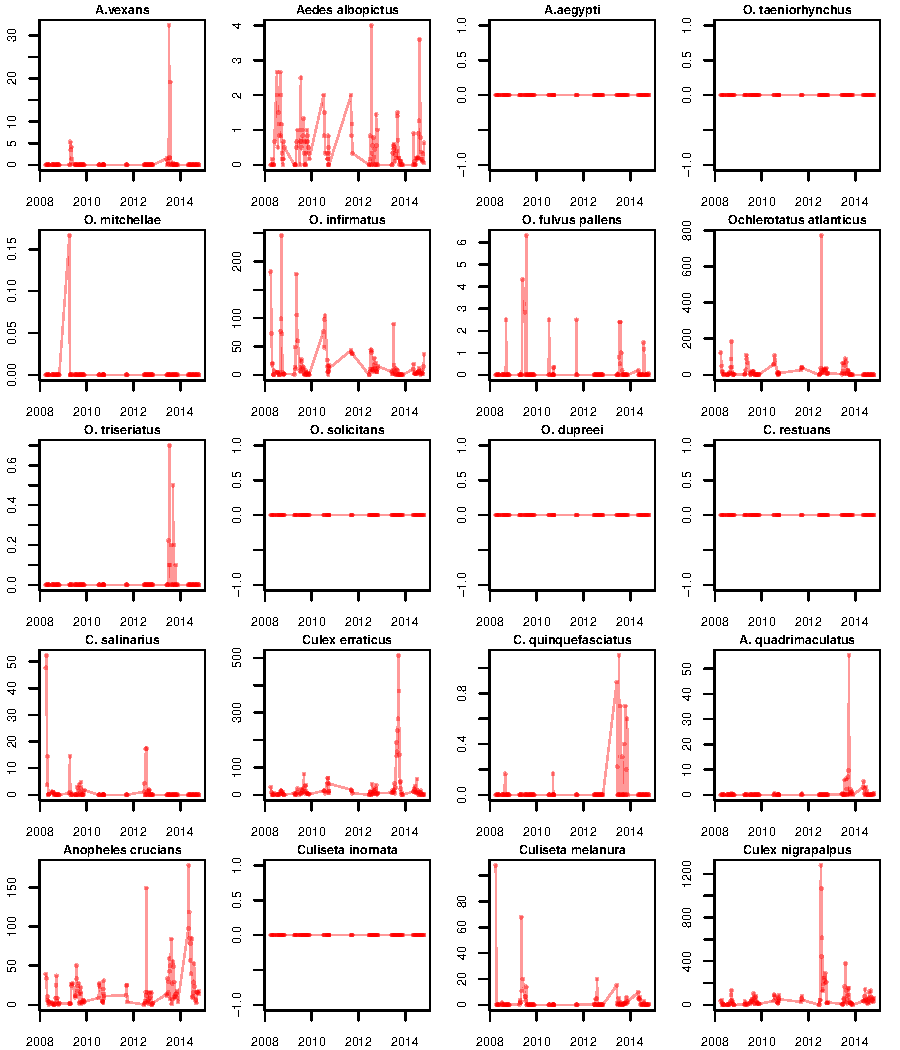
\includegraphics{mosquitoReport-009}


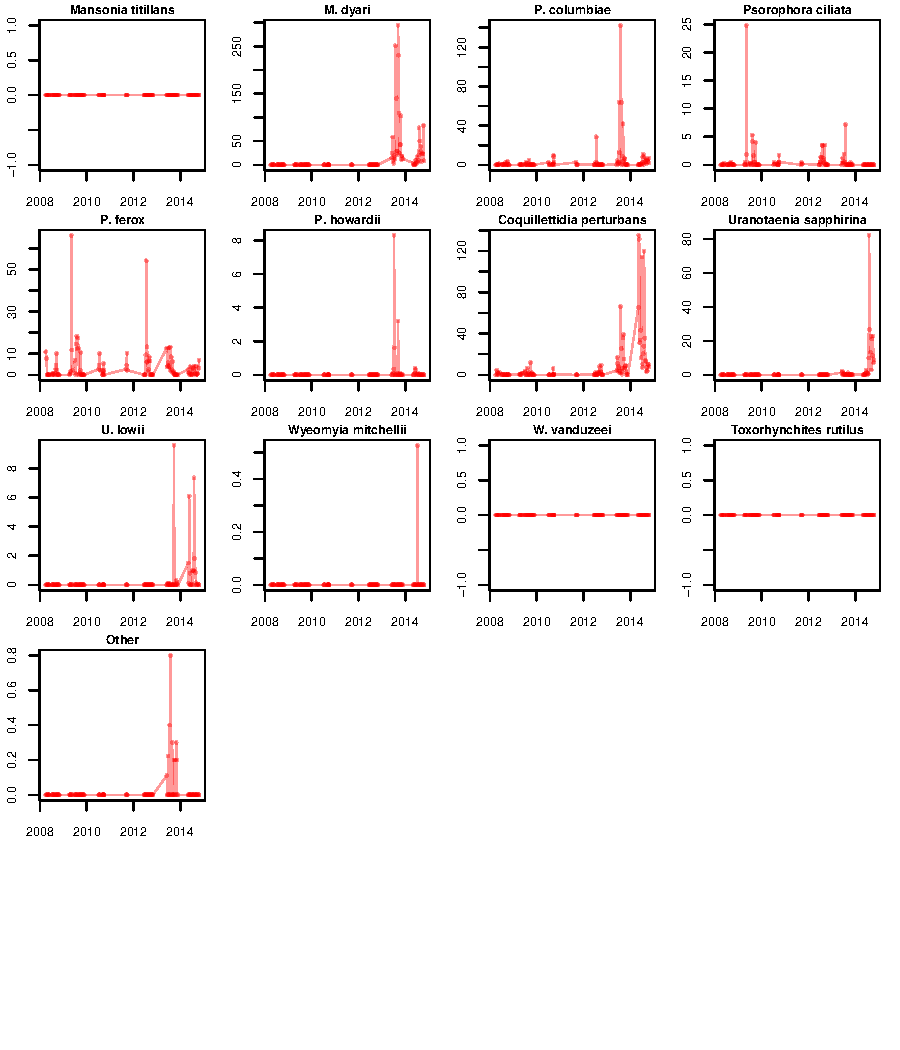
\includegraphics{mosquitoReport-010}




% \begin{multicols}{2} 
% \setkeys{Gin}{width=0.49\textwidth}

% \end{multicols}
% \setkeys{Gin}{width=1\textwidth}
% \end{adjustwidth*}





\newpage
%------------------------------------------
\section*{Details of Predictive Model}
\addcontentsline{toc}{section}{Details of Predictive Model}
%------------------------------------------
\hrulefill
\vspace{5mm}

Historically, the model has performed well, correctly predicting the late summer spikes in 2012 and 2013.  Given the preference for accuracy at high numbers, the model intentionally includes outlying high observations, thereby weighting them. \\

Having simulated more than 65,000 unique models, our best fit equation (using the sum of least squares approach) was: 

\begin{center} 
$\hat{Y} = \beta_0+ \beta_1^2 (5.6508)$ + \beta_2 (0.5938)$ 
\end{center}

\noindent where $\hat{Y}$ is the estimated mean number of mosquitoes per trap, $\beta_0$ is set to 0, $\beta_1$ is the cumulative rainfall in the period 15 to 29 days prior to the date of prediction and $\beta_2$ is the mean number of mosquitoes per trap in the most recent prior trap collection.  \\

Though an original model relied only on rainfall, incorporating the most recent trap predicition saw our R-squared improve from 0.52 to 0.82.  This means that we can now explain over 80\% of the variance in mosquito populations up to 15 days ahead of time.  





\end{document}
